\documentclass[12pt]{article}

\usepackage{upgreek}

\usepackage{amsmath}

\usepackage{graphicx}
\graphicspath{ {imgs/} }

\usepackage{dsfont}

\usepackage{hyperref}

\usepackage[utf8]{inputenc}

\usepackage{mathtools}

\usepackage{textcomp}

\usepackage[english]{babel}

\usepackage{tikz}

\usepackage{tcolorbox}

\usepackage{amsthm,amssymb}

\setlength{\parindent}{0cm}

\renewcommand\qedsymbol{$\blacksquare$}

\usepackage{fancyhdr}
 
\pagestyle{fancy}
\fancyhf{}
\fancyhead[LE,RO]{Graph Theory -- Fall 2017}
\fancyhead[RE,LO]{Joshua Concon}
\fancyfoot[CE,CO]{\leftmark}
\fancyfoot[LE,RO]{\thepage}


\begin{document}

\title{MATC32: Graph Theory\\ Lecture Notes}
\date{University of Toronto Scarborough -- Fall 2017}
\author{Joshua Concon}
\maketitle
Pre-reqs are MATB24, which is the second course on linear algebra at UTSC.
Instructor is Dr. Louis de Thanhoffer de Volcsey. I highly recommend sitting at the front since he likes to teach with the board. If you find any problems in these notes, feel free to contact me at conconjoshua@gmail.com.

\tableofcontents

\pagebreak

\section{Tuesday, September 5, 2017}

\subsection{The Seven Bridges of Konigsberg}

So basically there's this city called Konigsberg where a river flows through, and because of that, there are 7 bridges in the city. The bridges look like this:\\
\\
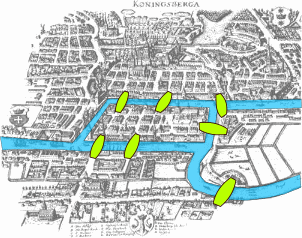
\includegraphics{Konigsberg_bridges}\\
\\

There problem that came up is whether or not it was possible to walk through every bridge in the city once in the same walk. This problem was eventually solved by Euler.\\
\\
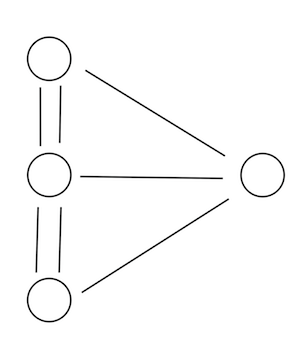
\includegraphics{Konigsberg_bridges_graph}\\
\\
It can be simplified to this. This is called a 'Graph', the circles are called 'nodes' or 'vertices' and the lines are called 'edges'. The different parts of the city are represented by the nodes and the bridges are represented by the edges.\\
\\
\begin{tcolorbox}[title=Definition: Graph ($G$)]
	\begin{enumerate}
		\item{Contains a set $V(G) =$ the set of nodes}
		\item{Contains a set $E(G) =$ the set of edges}
	\end{enumerate}
	A graph is called \textbf{Simple} if the graph has no loops and does not have multiple edges (i.e. Each edge is an unordered pair of distinct vertices).\\
	A graph is called a \textbf{Loop} if there is an edge that connects a vertex to itself.
\end{tcolorbox}

\begin{tcolorbox}[title=Definition: Path]
	A set of edges denoted by vertices $v_1, v_2, ..., v_n$ where there is a node between every edge between $v_i$ and $v_{i+1}$ $\forall i, 1 \leq i \leq n-1$
\end{tcolorbox}

\subsection{(Outline) Solution to Konigsberg}

Assume the graph has a path containing all edges $u_1,...,u_n$.\\
\\
Consider a vertex that isn't the first or last vertex travelled in the path (i.e. any vertex excluding $u_1$ and $u_n$).\\
\\
There must be an even number of edges for each of the nodes in between the edges in the path (excluding the first and the last node visited, unless the first and the last node visited are the same node).\\
\\
Since there are an odd number of adjacent nodes for all 4 nodes, this path does not exist. Therefore, there is no solution to Konigsberg.

\newpage

\section{Friday, September 8, 2017}

\subsection{Graphs}

\begin{tcolorbox}[title=Definition: Graphs]
	A graph $G$ consists of 2 (finite) sets:
	\begin{itemize}
		\item{$V(G)$ : vertex set}
		\item{$E(G)$ : edge set}
	\end{itemize}

	Together with an assignment from $E(G)$ to the set of subsets $V(G)$, where the subset is of size 1 or 2, containing the node(s) at the ends of the endpoints of each edge.
\end{tcolorbox}

If an edge has the same node at both of it's endpoints, it is called a \textbf{loop}.\\
\\
If 2 vertices are endpoints of more than one edge, we say that they are \textbf{multiply-edged}.\\
\\
A graph without multiply-edged vertices is called \textbf{simple}.\\
\\
\underline{Example:}

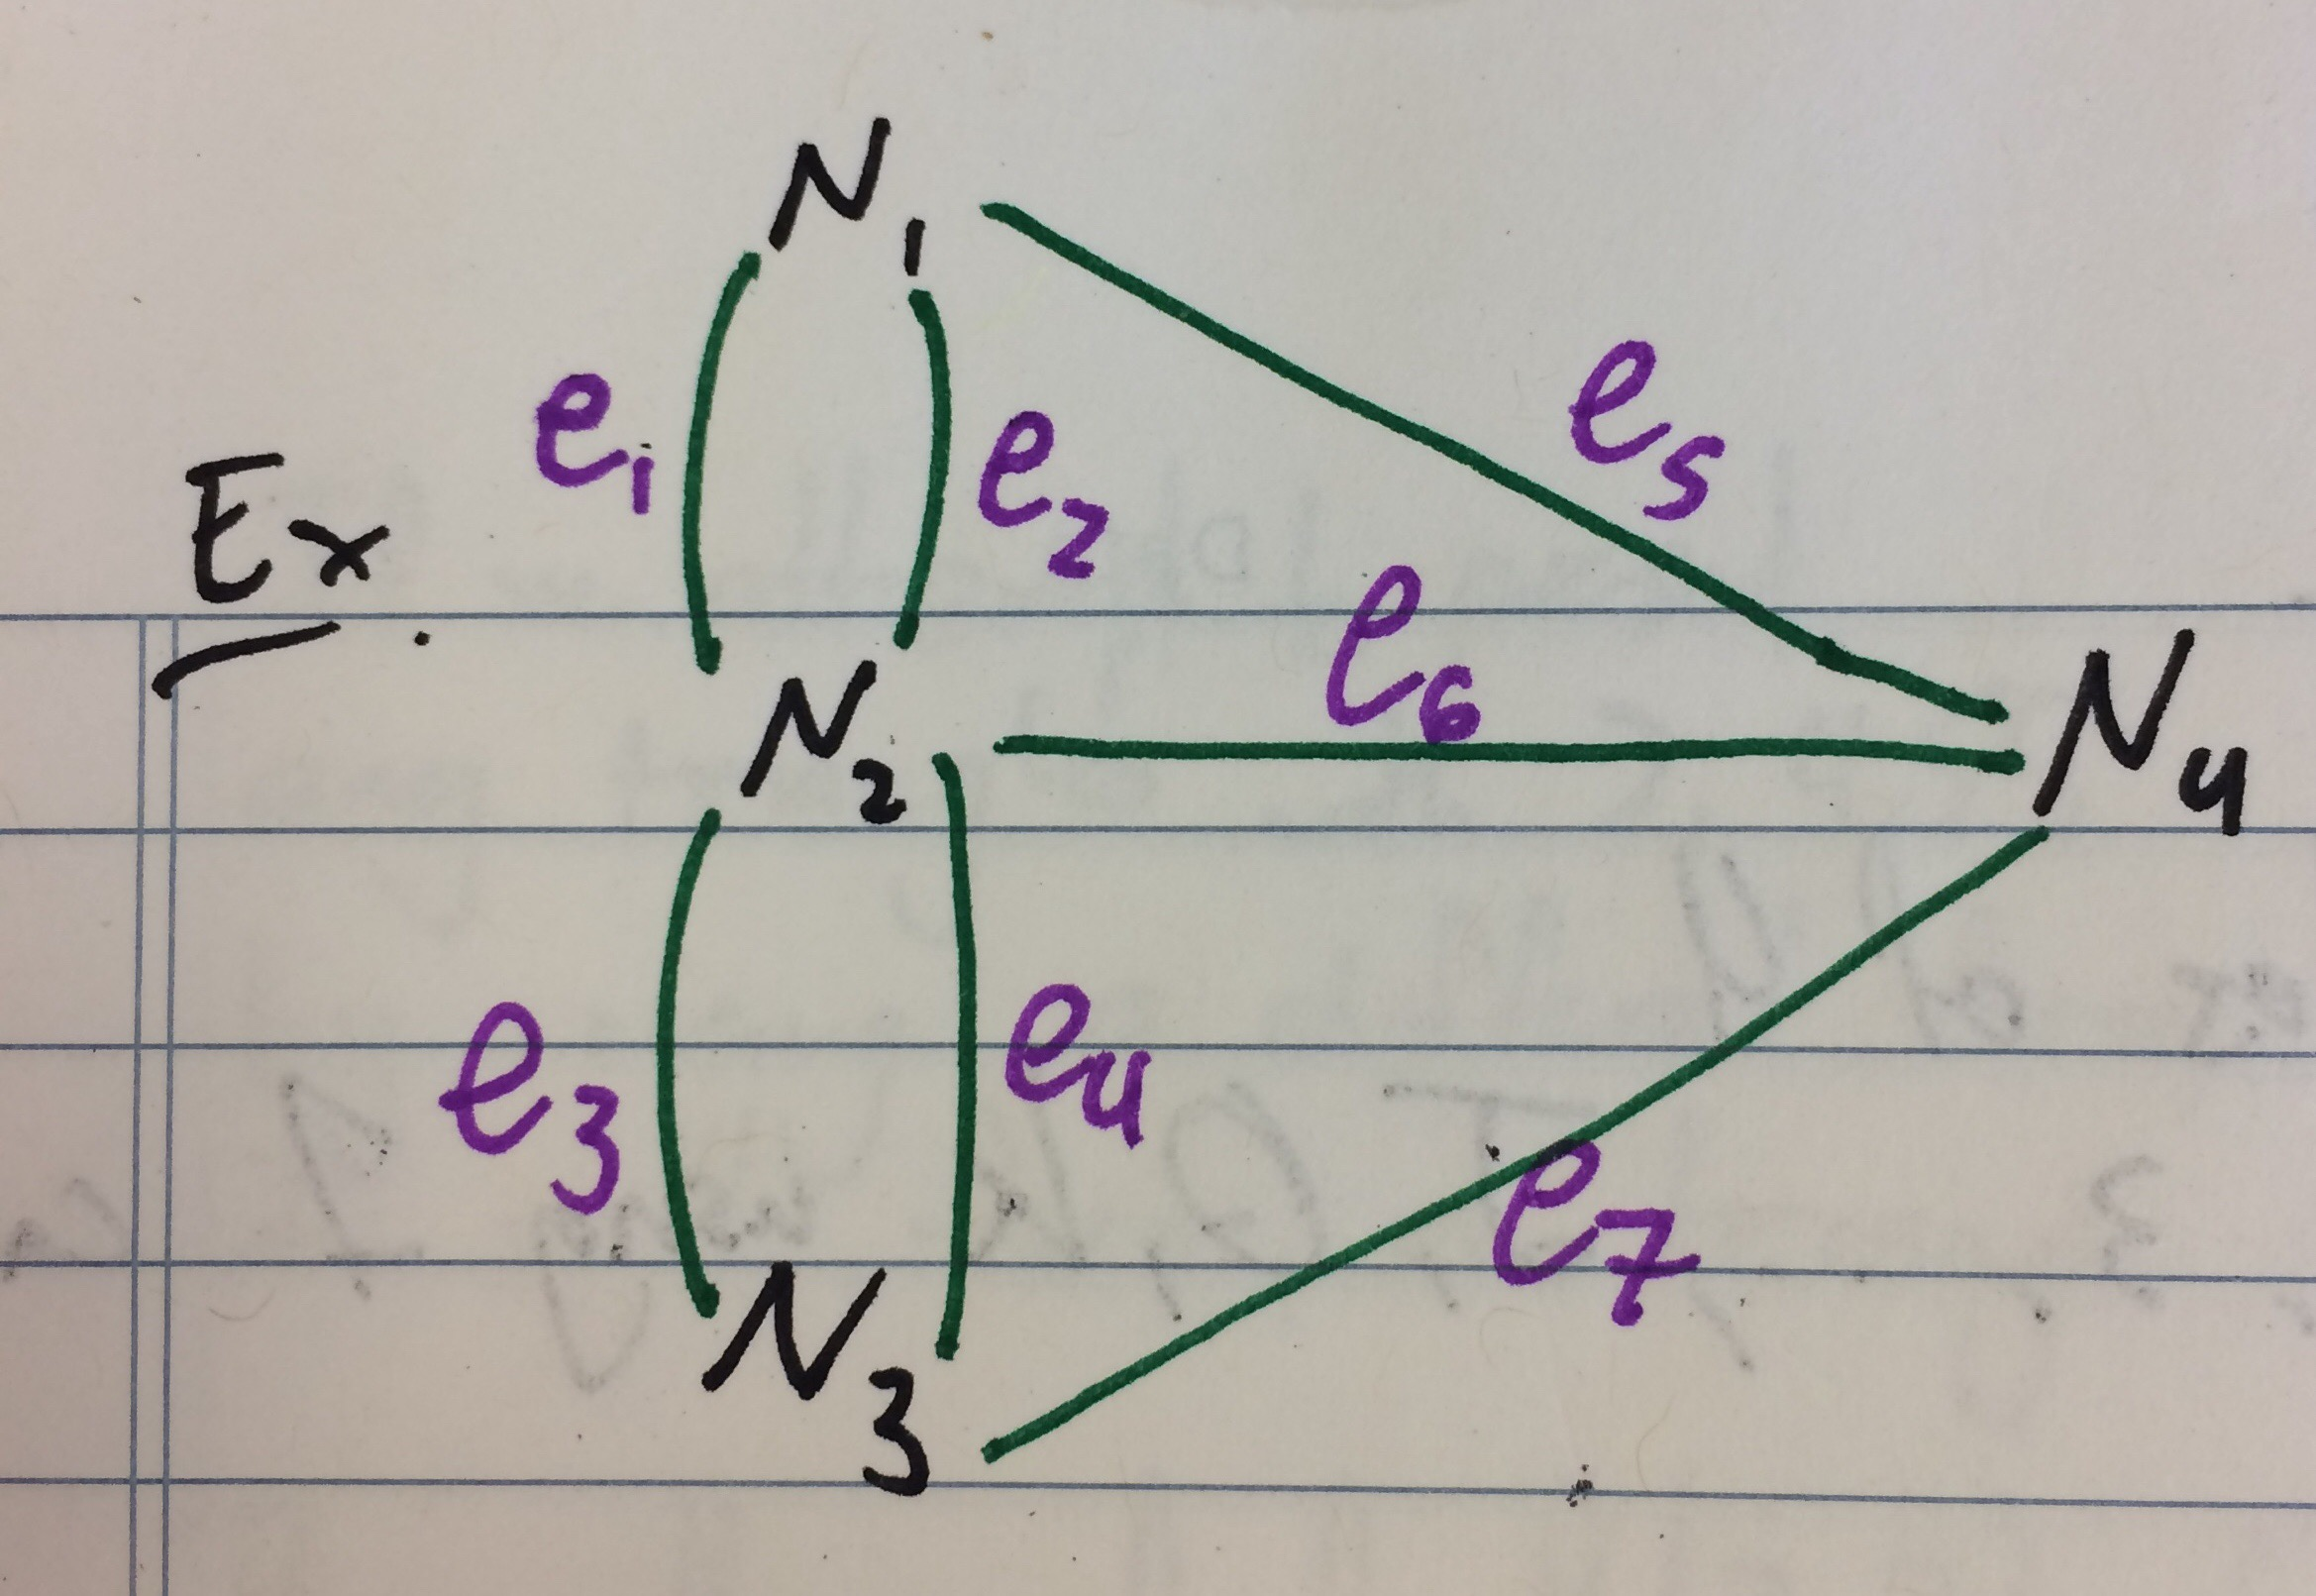
\includegraphics[scale=0.125]{lec2-1}

$$E(G) = \{ e_1, ... , e_7 \}$$
$$V(G) = \{ N_1, ... , N_4 \}$$

some of the assignments of $E(G) \mapsto V(G)$ include:
$$e_5 \mapsto \{ N_1, N_4 \}$$

\textbf{Adjacent edges} are edges with a vertex that is a common endpoint.

\subsection{Graph Theory Applications}

\subsubsection{Uber}

$$V = \text{People Using Uber (both drivers and passengers)}$$
$$E = \text{If it is realistic for a driver to pick up a person}$$

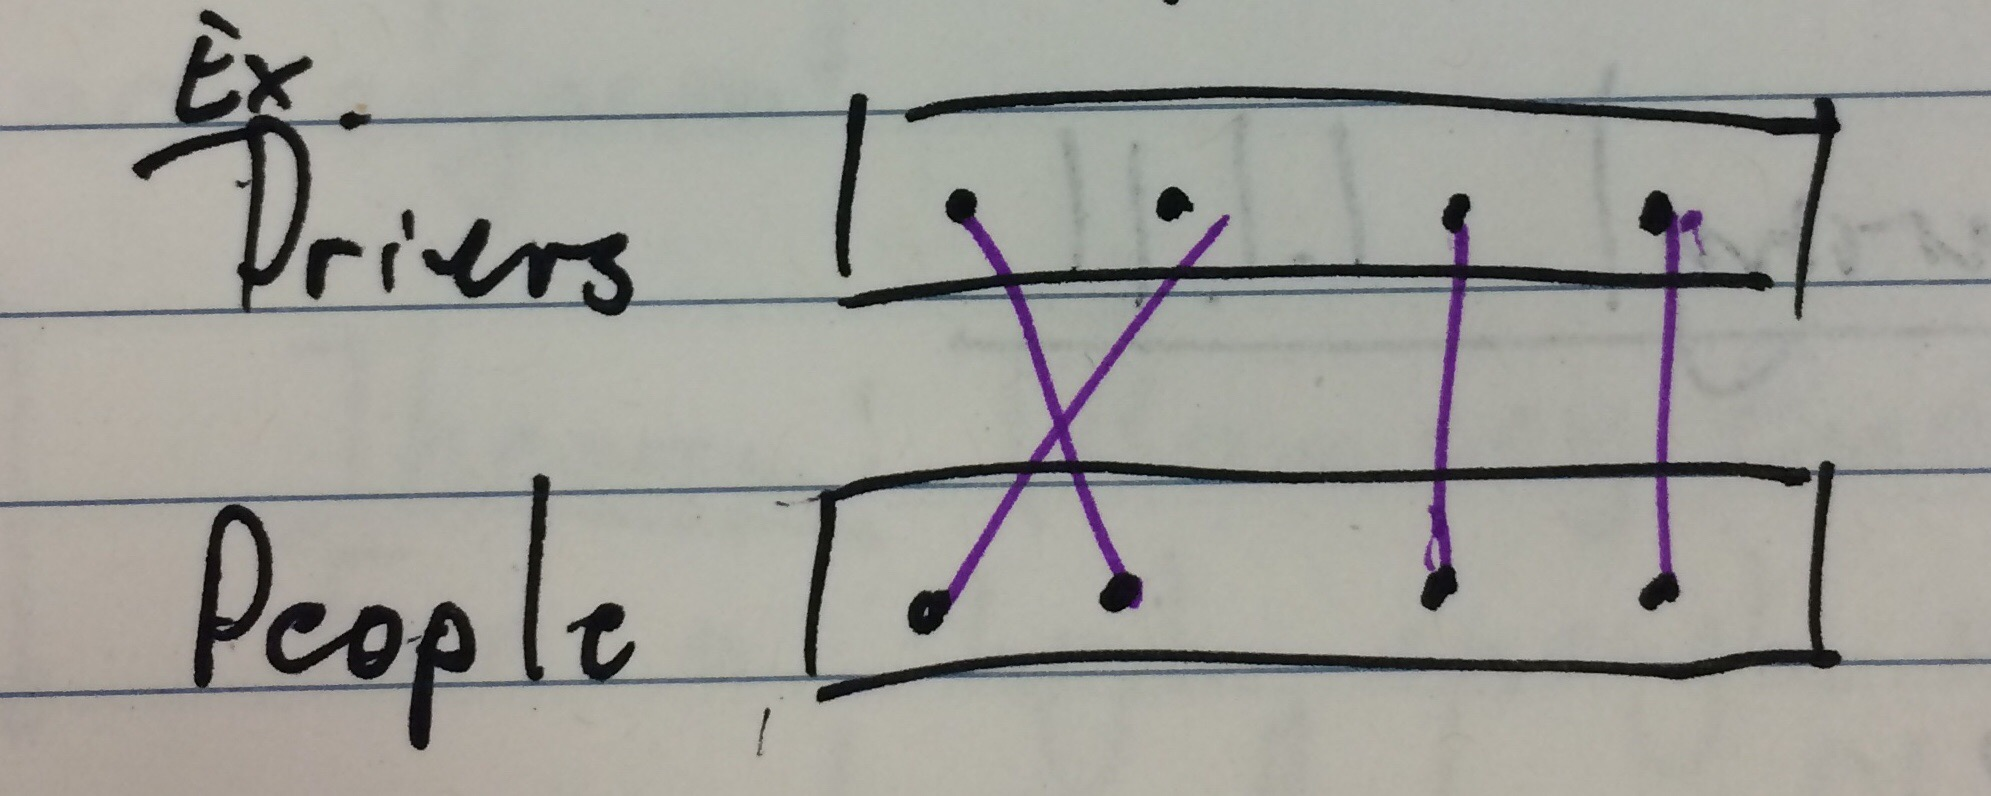
\includegraphics[scale=0.125]{lec2-2}

\begin{tcolorbox}[title=Definition: Matching]
	A \textbf{matching} in a group is a set of edges, none of which are adjacent
\end{tcolorbox}

\underline{Note:} $V(G) = S_1 \sqcup S_2$ and there are no edges between of $S_1$ with respect to $S_2$ ($\sqcup$ : refers to a union between two disjoint sets).\\
\\
These two sets $S_1, S_2$ are independent sets\\
\\
A \textbf{bipartite} graph has $V(G) = S_1 \sqcup S_2$ where both $S_1, S_2$ are independent.

\subsubsection{Monge's Theorem (on matching)}

Split a deck of 52 cards into 13 piles of 4, is it always possible to count an ace,2,3,...., Jack, Queen, King using 1 card drawn from each pile?

\subsubsection{Marriage (Stable) Problem}

Matching $n$ men with $n$ women


\end{document}


























